\section{Introduction} \label{sec:introduction}

Computer programs ultimately translate into sequences of individual operations.
These operations must specify the identities of registers and memory addresses they read from and write to.
Most modern programming languages introduce a layer of abstraction that specifies operands indirectly in terms of named variables and unnamed literal values.
As instances of computer programs by their very nature, genetic programs and digital artificial life systems must also specify computational operands on which to act.
These computational operands range from
\begin{itemize}
  \item program modules in genetic programs \citep{spector2011tag}
  \item virtual hardware analogs like registers, memory addresses, stacks, or jump addresses in genetic programs \citep{lalejini_tag-accessed_2019,ray1991approach,ofria2004avida},
  \item molecules in artificial chemistries \citep{bagley1990spontaneous},
  \item genes in artificial gene regulatory networks \citep{banzhaf2003artificial},
  \item individual neurons or neural modules in neuroevolution \citep{reisinger2007acquiring}, or
  \item agents in agent-based models of complex systems \citep{riolo2001evolution}.
\end{itemize}

In genetic programming, it is often essential for operations to undergo evolutionary adjustment to which computational elements they act on.
This capability can tweak the semantics of existing evolved code, critical in particular for duplication and divergence processes commonly highlighted in discussions of evolvability \citep{altenberg1994evolution}.
This capability also allows for incorporation of new computational elements and for removal of existing computational elements.
In genetic programming, dynamic reorganization of code modules can facilitate hierarchical problem-solving in genetic programming \citep{Kinnear:Koza:1994:adf}.
Similarly, reorganization and extension of existing computational elements is critical in the context of artificial life, where novelty and change are often of key interest \citep{taylor2016open}.

Tag-based referencing, sometimes also termed ``pattern matching'' or ``inexact referencing,' provides a practical solution for deciding computational operands.
This approach attaches a tag to each computational operand that may be selected and a tag for each querying operation.
Operand(s) are then selected for each query through a tag-matching process.
A querying operation's tag is compared to available operand tags.
Then, typically, either:
\begin{itemize}
  \item the best-matching operand is selected (e.g., \cite{spector2012tag}),
  \item all operands with match quality exceeding a threshold are selected (e.g., \cite{riolo2001evolution}),
  \item operands are activated to continuously-varying degrees based on match qualities (e.g., \cite{banzhaf2003artificial}), or
  \item operands are selected probabilistically based on match quality (e.g., \cite{seiden1992simulation}).
\end{itemize}

Inexact referencing facilitates orderly growth, shrinkage, and reconfiguration of a system's sets of operands and operations.
If an operand is deleted, it does not invalidate any existing operations, as other well-matching operands will fill its place.
Likewise, new operations can be created or existing operations can be altered freely without concern for potentially invalid operands.

John Holland's Echo model provides a motivating example for the use of tags in evolving systems \citep{holland1992adaptation, mitchell1994genetic}.
This complex adaptive system model revolves around agents competing over several renewable resources within a spatial grid.
Agents' life histories unfold through fighting, trading, and/or mating interactions with neighbors.
Equiping agents with the capacity to dynamically opt in or out of these exchanges based on neighbor identity was crucial to realizing the model's conceit to study emergent phenomena including ecology, economic exchange, and hierarchical organization.
To this end, each agent in the Echo model posesses a set of externally-facing ``appearance'' tags and a set of internally-held ``condition'' tags.
Tag matching regulates of agents' behavior: the occurance or non-occurance of each interaction stems from match quality between an agent's internal ``condition'' tag and the external ``appearance'' tag of its prospective partner.
Tag matching provides three major benefits.
First, interaction rules are well-defined between any possible paring of agents, even under dynamic insertion, removal, or mutation of agents within the system.
Second, agents can malleably and succinctly specify arbitrary sets of tag identities to allow or prevent interaction with.
Third, existing agent behavior can be adjusted or refined under mutation.

Indeed, inexact referencing techniques find common use in agent-based modeling \citep{riolo2001evolution}, neuroevolution \citep{reisinger2007acquiring}, artificial gene regulatory networks \citep{banzhaf2003artificial}, genetic programming \citep{spector2011tag, lalejini2018evolving}, artificial chemistry \citep{dittrich2001artificial}, and artificial immunology \citep{timmis2008theoretical}.
These systems typically either use tagging schemes based on
\begin{itemize}
    \item Hamming distance between bitstrings (\textit{e.g.}, \cite{lalejini2018evolving,banzhaf2003artificial}) or
    \item differences between real-valued scalars (\textit{e.g.}, \cite{riolo2001evolution,spector2011tag}).
\end{itemize}
However, other nonlinear tag-matching systems, such as Downing's streak metric \citep{downing2015intelligence} and de Boer's adjacency match metric \citep{DEBOER1991381}, have been proposed.
Incorporation of a wildcard ``match-any'' character into tag alphabets has also been proposed \citep{holland2012signals}.

Although some efforts have been made to distinguish certain tag-matching criteria in terms of narrative explanations of their evolutionary properties and appeals to biological analogy \citep{downing2015intelligence,scherer2004activation}, no work has yet provided systematic, quantitative, and empirical insight into the ramifications of tag-matching criteria.

We hypothesize that properties of tag-matching criteria could potentially affect evolvability through mechanisms including
\begin{itemize}
  \item bias of certain queries or operands against tight-affinity matches (i.e., tunable specificity)
  \item bias to the stability of certain connections under mutation (i.e., tunable robustness),
  \item bias to the likelihood of connections arising between subsets of queries and operands (i.e., modularity), and
  \item mitigation of disruption under duplication of queries and operands (i.e., gene duplication \citep{ohno2013evolution, lewis1978gene}).
  % found these classic gene duplication references here: https://www.sciencedirect.com/science/article/pii/S108495219990335X
\end{itemize}

In this work, we survey five tag-matching schemes: two based on integer representations, one based on Hamming distance, a "streak" metric based on the maximum length of identical substrings, and a control metric that uses a hashing algorithm to compute completely arbitrary match distances.

We explore how these tag-matching schemes differ with respect to
\begin{enumerate}
  \item geometric structure that biases or limits the patterns of connectivity that form among queries and operands (Section \ref{sec:geometric}),
  \item variational properties that influence changes to connectivity observed under mutation (Section \ref{sec:variational}), and
  \item evolutionary outcomes such as the rate of adaptive evolution and the quality of evolved solutions (Section \ref{sec:evolutionary}).
\end{enumerate}

Across several geometric analyses, we found the geometric structure of the integer metrics to be most restrictive, followed by the Hamming and then streak metrics.
We observed large-effect one step mutations under the integer metrics and streak metrics, but not under the hamming mutation.
Except for the control hash metric, match affinity decayed most rapidly along mutational walks under the integer metrics.
Match affinity decayed slowest along mutational walks under the hamming metric.

Evolutionary experiments also showed meaningful differences between tag-matching schemes.
We found that rigid, one-dimensional geometric structure of the integer metrics impeded satisfaction of multiple simultaneous tag-matching requirements in scenarios where a query tag was required to closely match to more than one operand.
Integer metrics also fared poorly in genetic programming experiments, even when the selected-for tag-matching scenario only involved matching queries to a single operand.
Evolutionary conditions in these experiments were configured to emphasize duplication and divergence by restricting sources of variation, namely initial tag variation and ongoing insertion of randomly-generated tags.
The Hamming and streak metrics generally fared best, with the streak metric outperforming the Hamming metric in some scenarios.

Although the Hamming and streak metrics generally matched or outperformed the integer metrics, confirming the extent to which these findings generalize across tag-matching application domains beyond those surveyed --- particularly with respect to mutation operator used --- necessitates further research.
Improved understanding of the implications of tag-matching rules will directly enable more effective genetic programming practice.
To a more theoretical bent, this work also provides a foundation for inquiry into the properties and mechanisms of tag-matching systems in nature.

In support of further investigations, all tag-matching techniques compared here were incorporated into the open-source Empirical C++ library \citep{charles_ofria_2019_2575607} as interchangeable components of the MatchBin tool suite.

%Although some work has been done comparing the , for example minimum match-quality cutoff threshold \citep{lalejini2019} and selection \citep{Moreno_2019}
%The implications of underlying criteria determining tags' affinities have been unexplored.
%Here, we characterize meaningful differences among tag-matching systems with respect to geometric, variational, and evolutionary properties.


% of tag-matching systems.
% Such findings will be of practical use May raise interseting evolutionary/theory questions.

%In this work, we set out to characterize several tag-matching schemes between bitstring tags that have been proposed in the artificial life and genetic programming

% We overview the bitstring tag representation and the tag-matching metrics that we used in our experiments.
% Paper layout

% neuroevolution

% gene regulatory networks \citep{}

% artifical life: tierra  for program flow control nops

% \citep{bagley1990spontaneous} probability of reaction or reaction rate


% Spector et al. pioneered the use of tag-matching schemes in genetic programming (GP).
% In \citep{}, Spector et al. use an integer-based tagging and tag-matching to retrieve data items from PushGP stacks, including code modules (TODO @amlalejini is this right?). % @AML: more or less, yes that's right
% @AML: Work in mention of tag-access memory? Want to advertise the technique so that someone else can come along and try it out in more contexts\ldots this might not be the best place to do so, though.
% Additional work extended the use of tags for labeling and referring to positions in memory \citep{lalejini_tag-accessed_2019} for linear GP systems.

% In existing work, the event-driven genetic programming representation SignalGP has used a Hamming-distance-based tag-matching scheme to activate program modules in response to tagged events.
% In , Lalejini and Ofria demonstrate the event-driven paradigm realized with tag-matching yields better-performing evolved solutions to an environmental state tracking problem and a distributed leader-election problem.
% In \, Lalejini and Ofria investigate the consequences of applying a .
% Requiring exact or near-exact matches cripples the rate of adaptive evolution against the environmental state tracking problem, ostensibly because the probabilities of establishing event-module connections through mutation becomes miniscule.
% On the other hand, enforcing only a low match-quality quality cutoff threshold reduces the quality of evolved solutions in the presence of additional irrelevant environmental cues.

% Spector et al. use an integer-based tagging system, while Lalejini and Ofria use a Hamming-distance based tagging system.
% In \citep{downing2015intelligence}, Downing proposes a tag-matching metric based on the lengths of matching and mismatching streaks between two bitstrings but does not demonstrate it in an evolving system.
% (We formally characterize these tag-matching systems in our Methods section.)


%Metric dimensionality constrains the possible relative orderings of matches.
%A one-dimensional metric can represent all possible query-to-single-operand lookups.
%However, it can not represent all possible query-to-multiple-operand lookups
%This, of course, is relevant to a system where a query matches with multiple operands.
%In a dynamically matched query-to-single-operand system, however, this can be relevant to the resulting connectivity under runtime silencing or upregulation of modules.
%However, even in a static system, this can be relevant to resulting connectivity under deletion of an operand.

%Figure \ref{fig:1d-2d-single-double} provides an example of a set of two-match orderings that a one-dimensional metric, like the integer metric, cannot represent.
%\begin{figure}
\begin{center}

\begin{subfigure}[b]{\columnwidth}
\centering
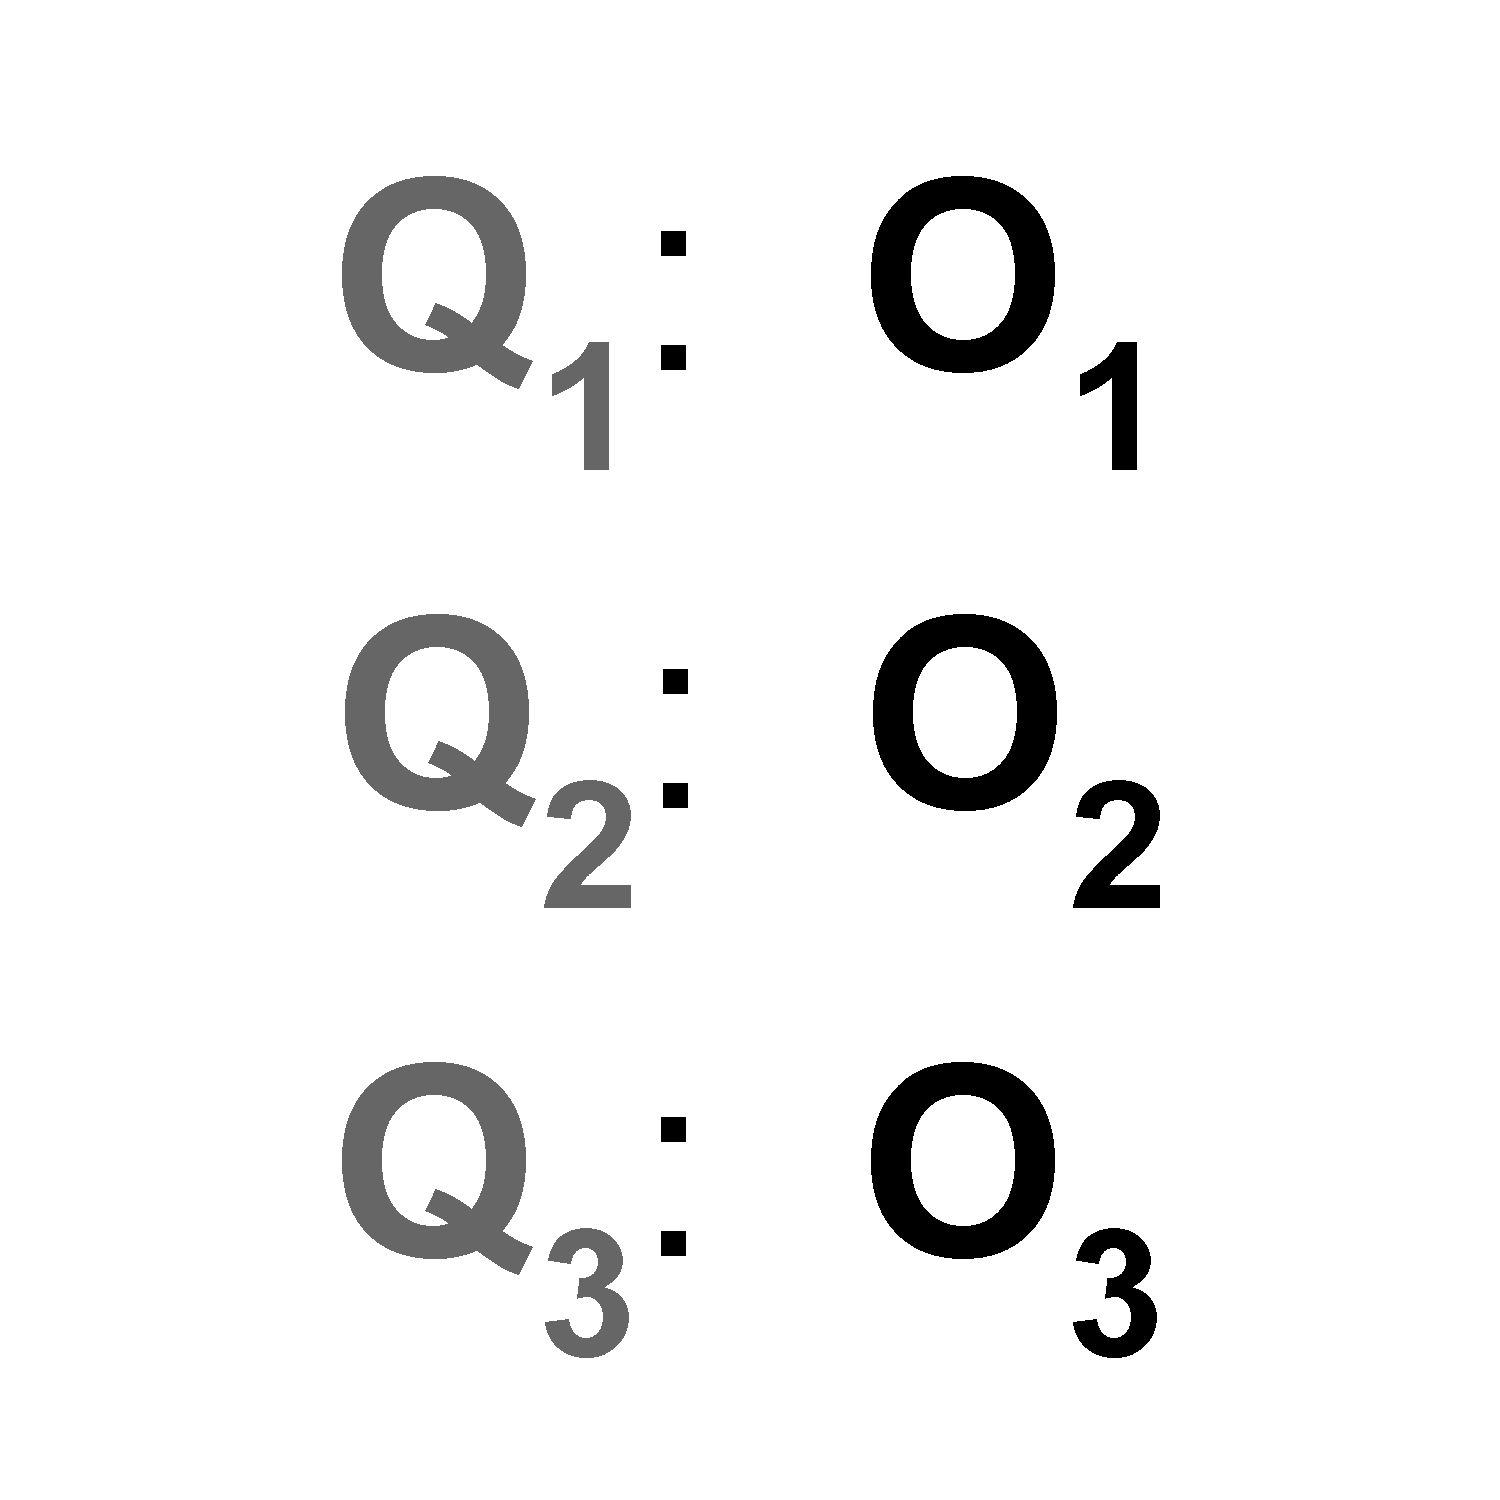
\includegraphics[width=0.33\columnwidth]{{{1d-2d-single-double/single}}}%
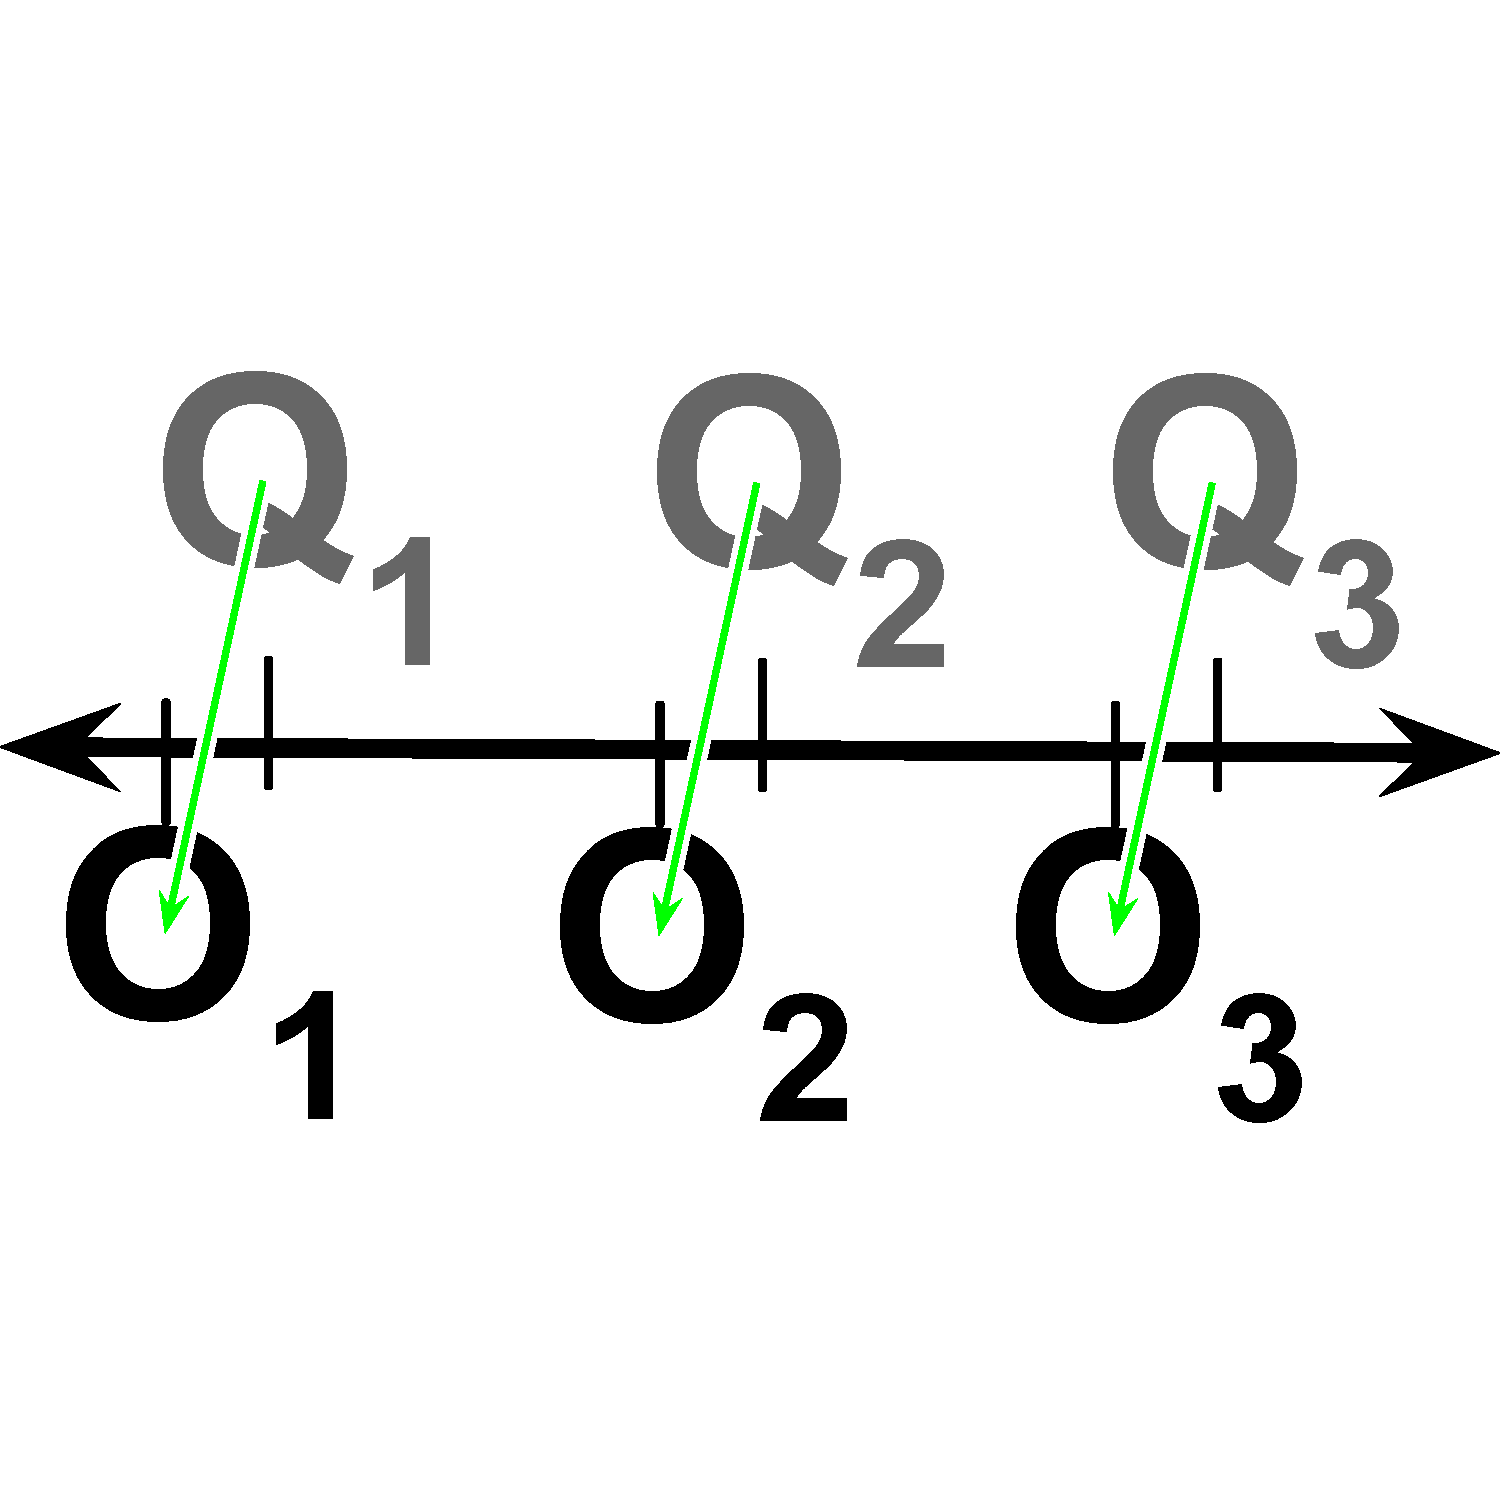
\includegraphics[width=0.33\columnwidth]{{{1d-2d-single-double/1d-single}}}%
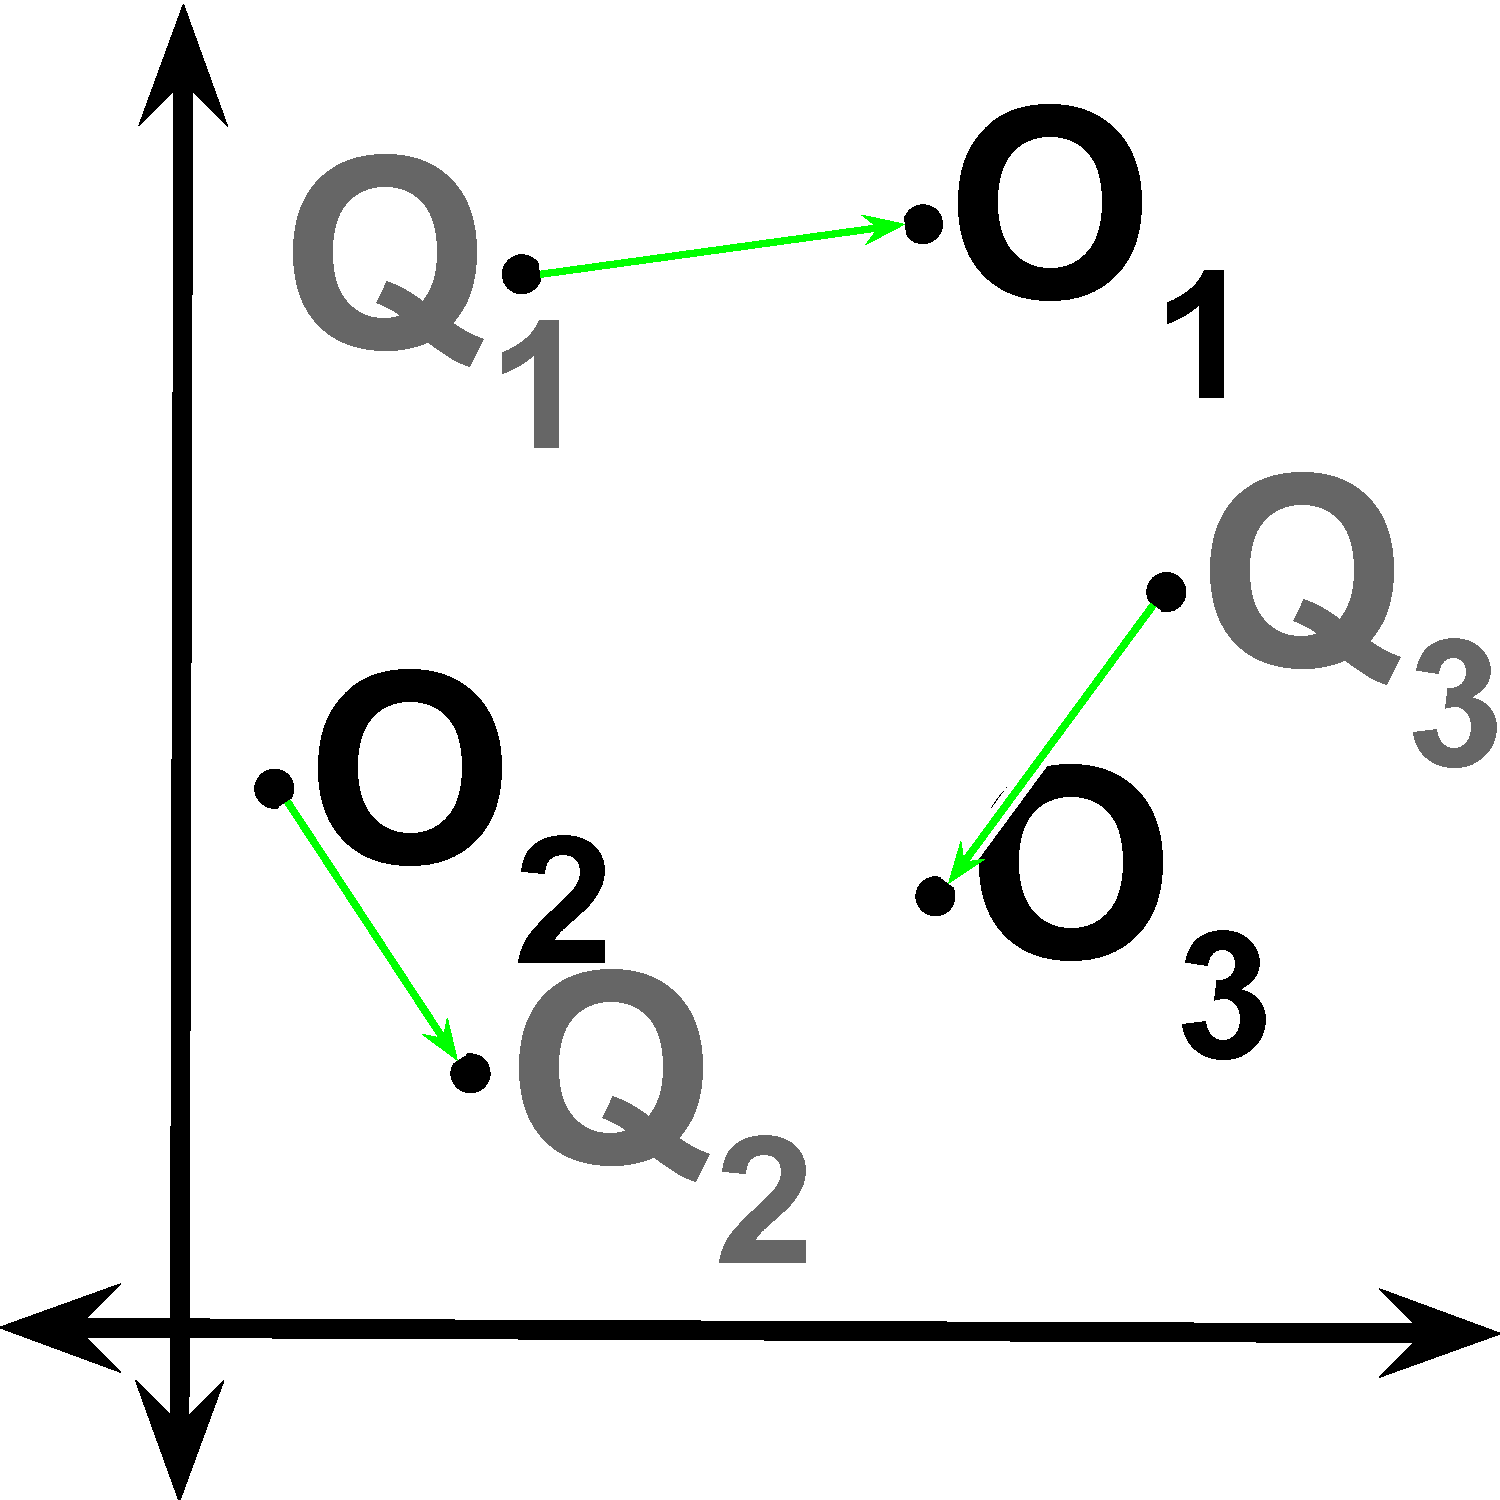
\includegraphics[width=0.33\columnwidth]{{{1d-2d-single-double/2d-single}}}
\caption{
Single-operand matching constraint
}
\label{fig:single}
\end{subfigure}

\begin{subfigure}[b]{\columnwidth}
\centering
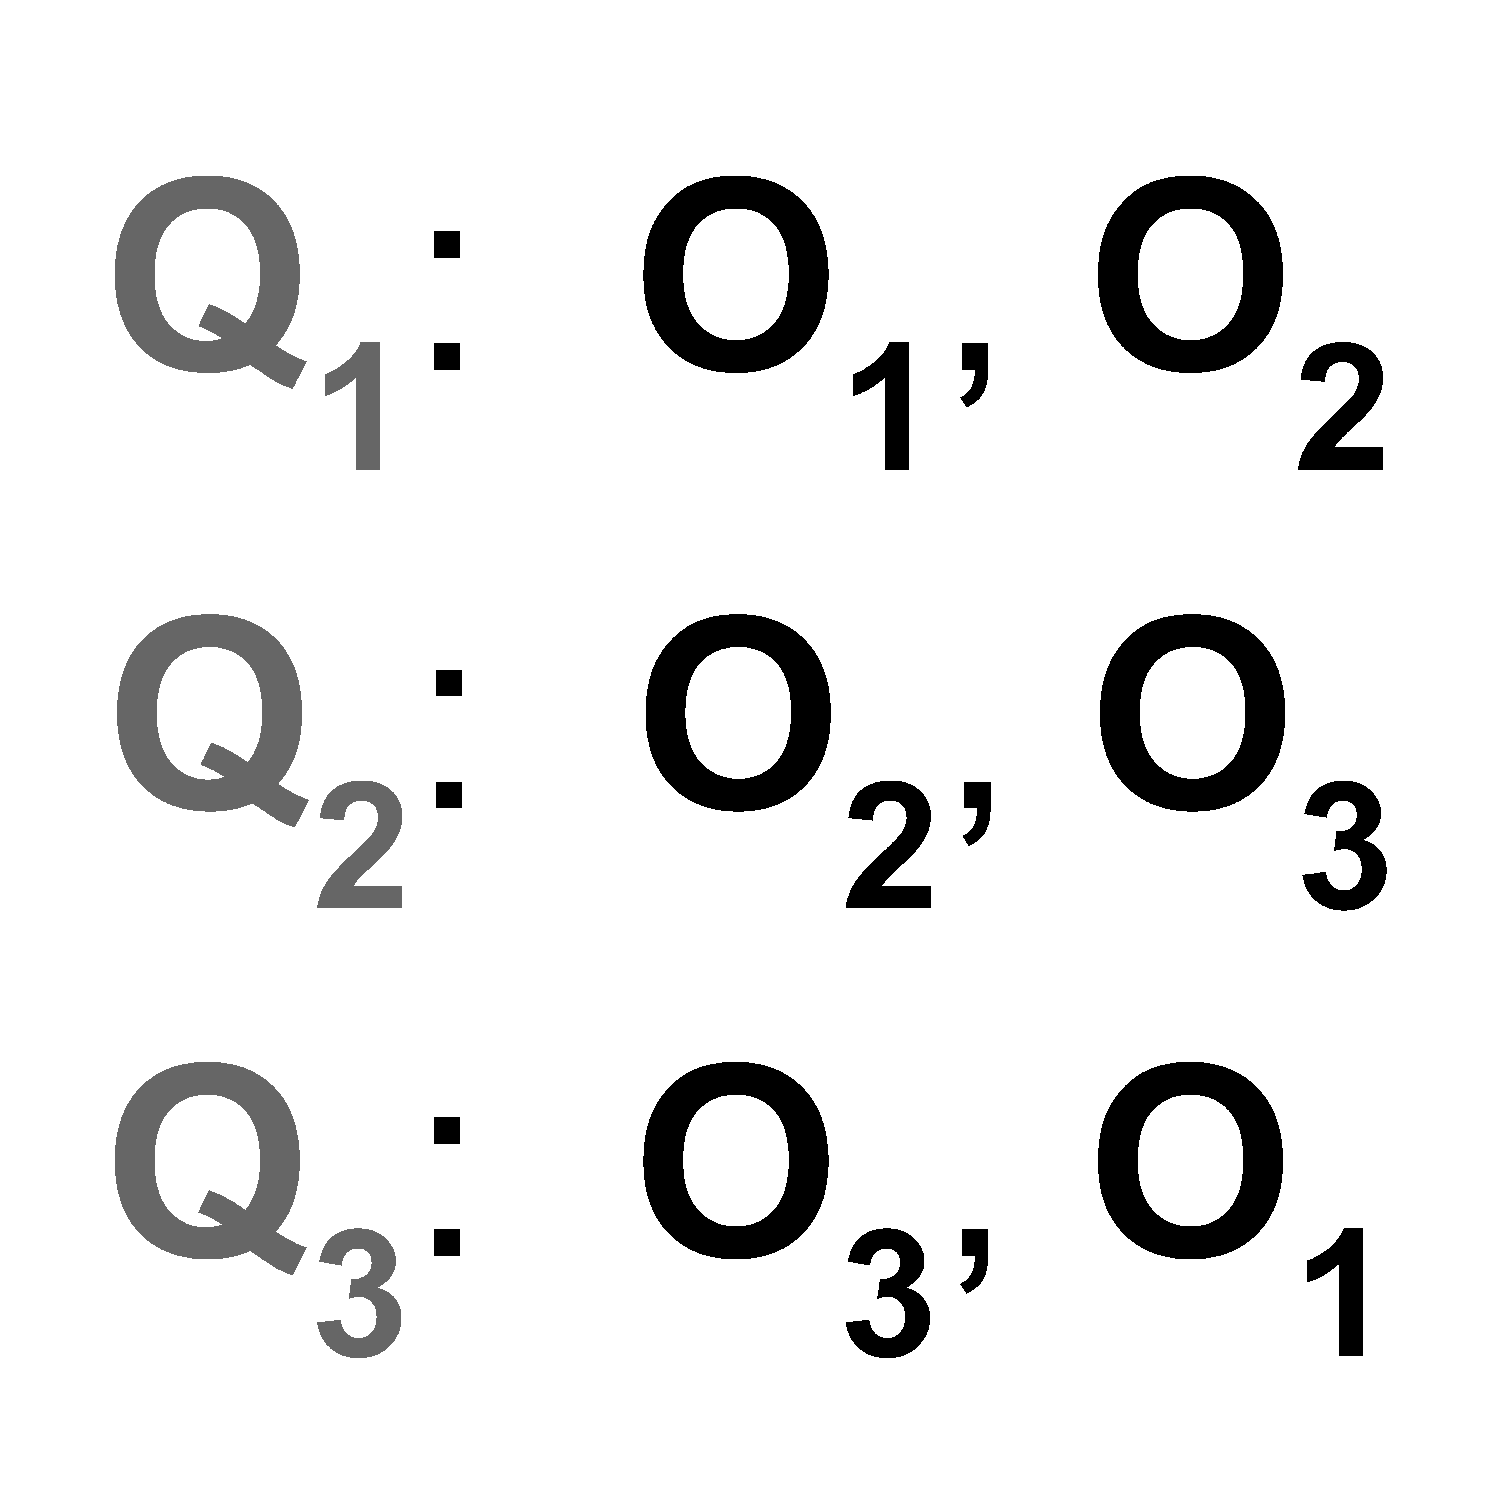
\includegraphics[width=0.33\columnwidth]{{{1d-2d-single-double/double}}}%
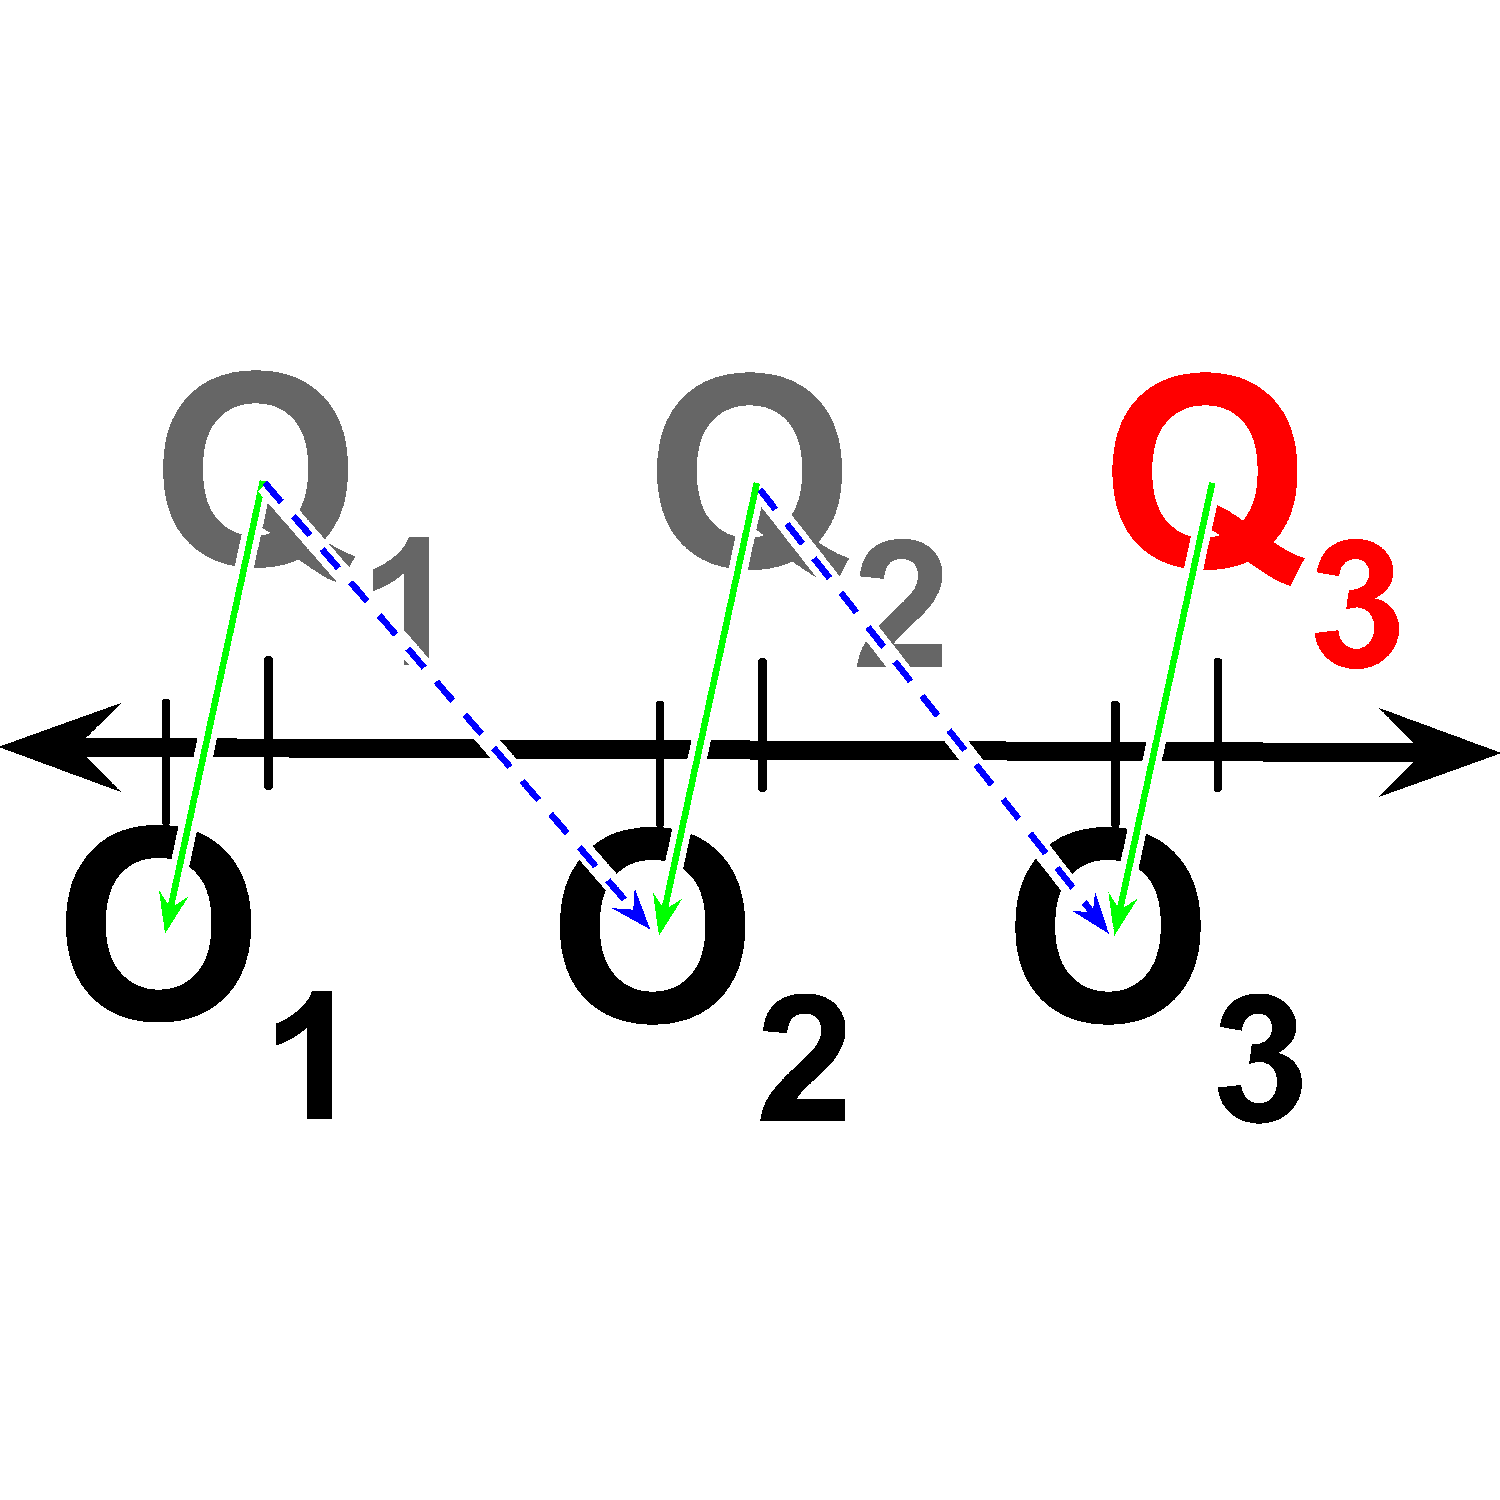
\includegraphics[width=0.33\columnwidth]{{{1d-2d-single-double/1d-double}}}%
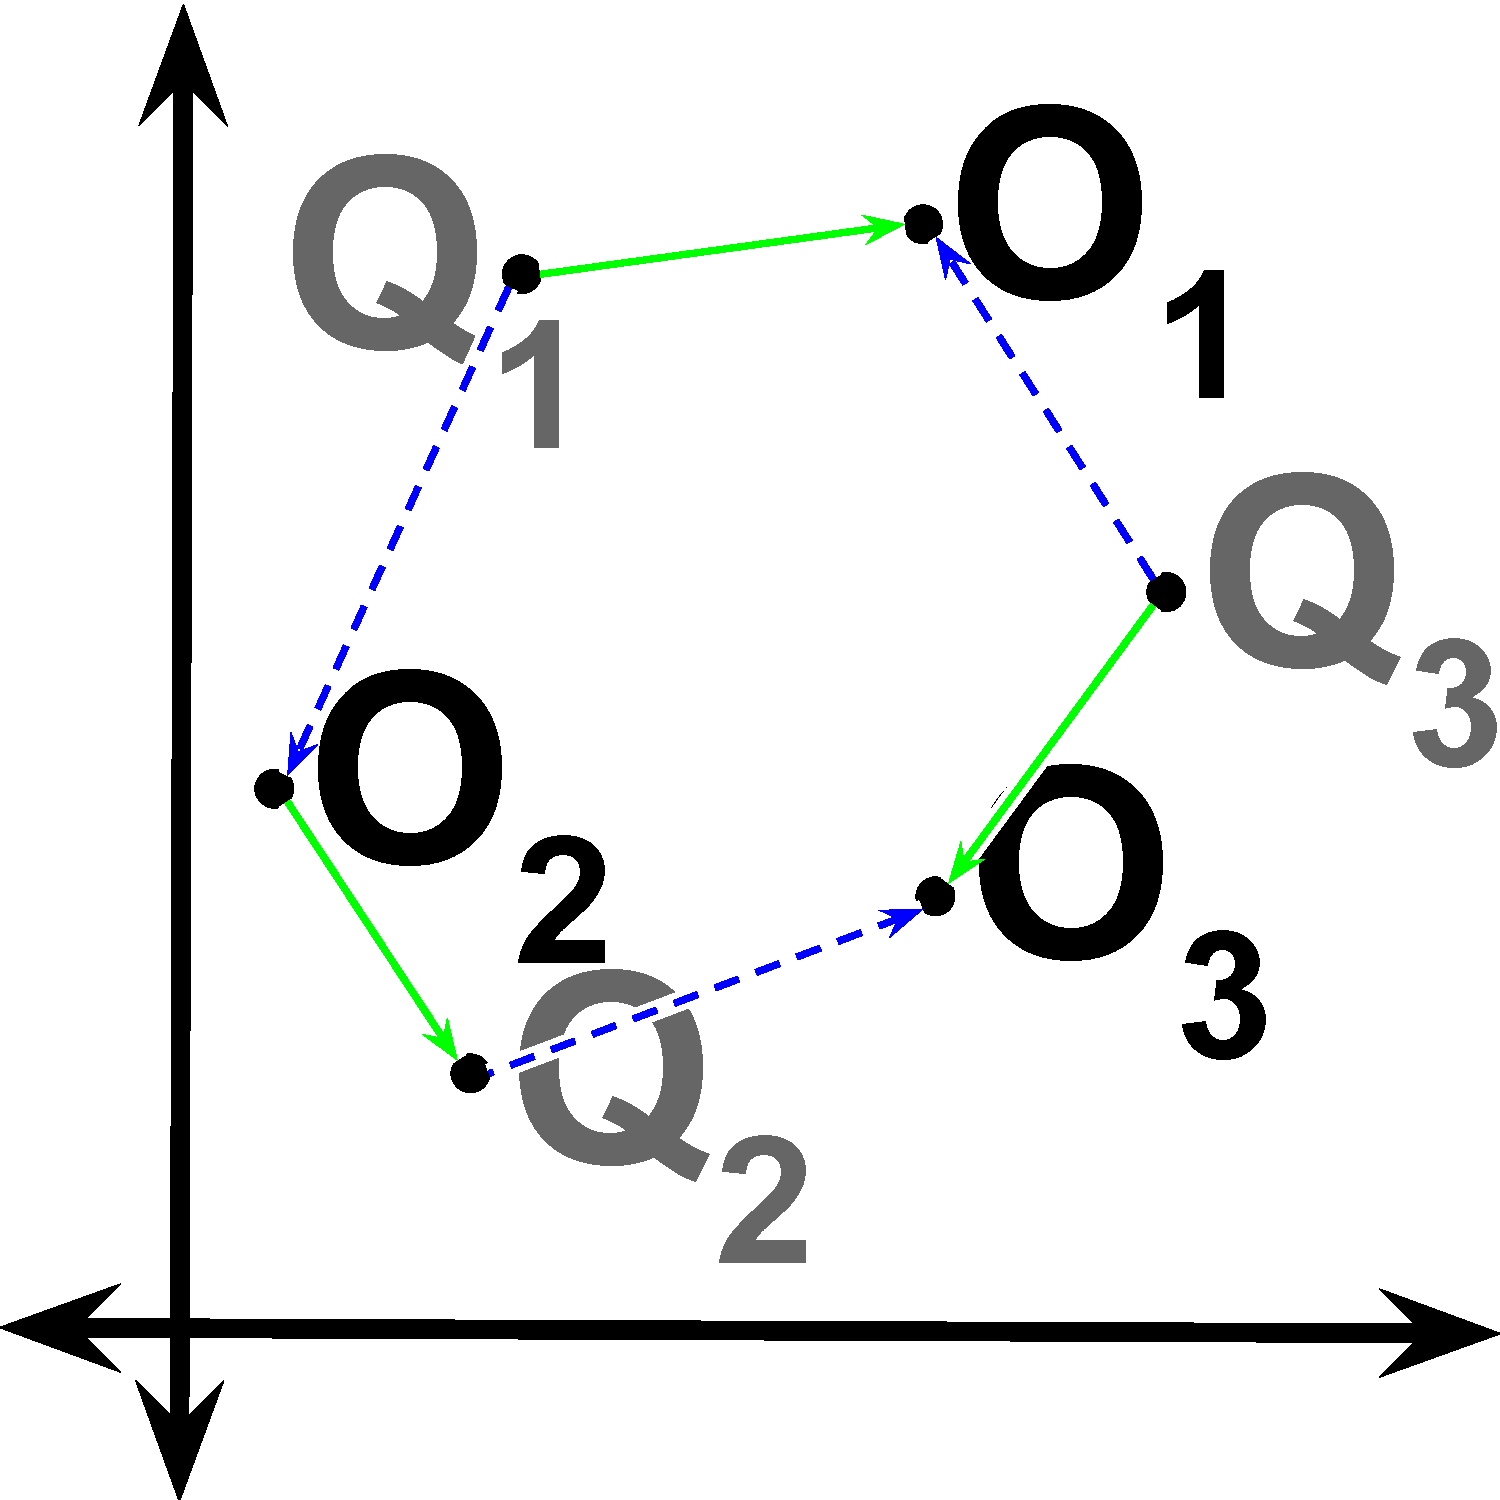
\includegraphics[width=0.33\columnwidth]{{{1d-2d-single-double/2d-double}}}
\caption{
Double-operand matching constraint
}
\label{fig:double}
\end{subfigure}

\caption{
A cartoon depicting the necessity of tag space dimensionality to satisfy multi-operand matching constraints.
}
\label{fig:1d_2d_single_double}

\end{center}
\end{figure}

%Even higher-dimensional metrics are necessary to represent arbitrary longer-match orderings.

%Metrics also differ in their respect for the triangle inequality, that $d(a,c) \leq d(a,b) + d(b,c)$.
%Consider a system in which close matches $d(Q_1, O_2) < t$ and $d(Q_1, O_2) < t$.
%Where also $d(Q_2, O_2) < t$ but $d(Q_2, O_1) > 3t$.
%This is not possible if the triangle inequality holds because we would have $d(Q_2, O_1) < d(Q_2, O_2) + d(Q_1, O_2)+ d(Q_1, O_1) < 3t$.
%Very sad if $3t$ is the similarity threshold for ignoring!
%A similar example can be constructed for a threshold where everything matches (TODO can it?).

%This and also commutativity is also a potentially relevant concern in systems (such as artificial chemistries) where the set of queries and the set of operands are one and the same.

%Tag-matching systems also differ with respect to variation induced under tag mutation.
%A pair of tags matched using the streak metric may both contain neutral sites (e.g., sites not involved in a matching or mismatching streak between the tags) that can mutate freely with no effect on match quality.
%In contrast, a pair of tags matched using Hamming or integer metrics contain no neutral sites: every mutation affects match quality.

%Likewise, every individual mutation on a pair of tags matched using the Hamming metric has an effect of equal magnitude on match quality.
%However, an individual mutation on a pair of tags matched using the streak metric may have no effect on match quality (e.g., a neutral site), a slight effect on match quality (e.g., on the periphery of a matching or mismatching streak), or a severe effect on match quality (e.g., at the center of a matching or mismatching streak).

% The evolutionary consequences of a tag-matching scheme's underlying similarity-defining metric remain unexplored.
% Do different tag-matching metrics exhibit different rates of adaptive evolution?
% Do tag-matching metrics affect the quality of evolved solutions?
% If so, which tag-matching metrics best promote rapid adaptive evolution and high-quality evolved solutions?
% And under what circumstances?

% literature.

%First, we examine geometric properties of the tag-matching schemes: how do TODO?

%Then, we analyze variational properties of the tag-matching schemes: how do TODO?

%We run a toy target-matching evolutionary experiment to see if these geometric and variational properties have an effect in practice.

%Finally, we throw the different tag-matching schemes into a to test them on diagnostic problems that weren't specifically designed for tag analysis.


%In traditional computer programming, computational elements are
% what about indices


% Mutation of names, addition or removal of modules at run time.
% Expressed in terms of the abstractions artificial life systems: from virtual hardware stand-ins like registers, stacks, or jump addresses in genetic programs,  in artificial chemistries, genes in gene regulatory network models, individual neurons or neural modules in neuroevolution, or more-general specification of agent interactions in agent-based models of complex systems
% // has a ton of ciatations for agent interations in agent-based models of complex systems: https://www.sciencedirect.com/science/article/pii/S0950705116302994

% In traditional computer programming, BLAH

% The creation of novel elements, the extinction or removal of elements,


% We will refer to computational elements that are specified among by a computer program as operands.
% The term queries will describe sites in the computer program where a operand is specified.

% As instances of computer programs, genetic programs must also specify computational elements on which to act.
% Several approaches to addressing this problem have arisen.

% % @AML:
% % - Some existing addressing mechanisms in GP: (1) direct addressing (enumerating all possible operands, encode in query), (2) type-based addressing (PushGP stacks), (3) probabilistic addressing (e.g., recent tangled program graph shared memory mechanisms), (4) template-based addressing (avida, tierra).

% Operands may be implicitly specified according to the position of a query in a genetic program.
% Tree-based GP, which traditionally represent programs as a rooted binary trees of operations, exemplify this approach.
% An operation's inputs are simply the outputs of its child nodes.
% %Lones and Tyrell commmentary: mutational operator disaster
% %potentially restricts possible topologies?

% A second possibility is to enumerate all possible operands, assign each a operand unique identifier, and then encode an identifier for each query.
% However, this approach doesn't effectively support the addition or removal of operands.
% %* too many options first = miniscule probability of connecting
% %* too few options next

% Tag-matching constitutes a third possible solution.
% This approach encodes a tag for each query and for each available operand.
% Then, operands are specified for each query through a tag-matching process where the query tag is compared to all available operand tags and the best-matching operand is selected.
% Queries may be dereferenced prior to program evaluation (e.g., static) or during program evaluation (e.g., dynamic), potentially allowing for program state to influence which operands are specified by queries.
% This third idea is similar to the second except that it allows for the number of operands to change without the need for a complicated and potentially arbitrary mutation operator to update invalidated queries.

% %Duplication and deletion of genes (e.g., modules) is important in evolutionary biology in the evolution of complex features (TODO cite).
% %Genetic program representations that accommodate such events might help GP benefit from these events .
% What are the benefits of tags/tag-based referencing?

% \begin{itemize}
%   \item Hypothesis: Inexactness allowed by tag-based referencing makes these references
%         more robust to minor genetic perturbations, smoothing the genotype-phenotype
%         mapping relative to more traditional memory-indexing techniques (pulled from
%         2019 Tag-access memory abstract).
%   \item We don't need to know/lock-in the architecture of what our tags are referencing.
%         If a referent (e.g., module) is deleted, it doesn't invalidate any of the
%         in-program references (e.g., module calls). The same is true for creating
%         a new referent. For example, using tags to reference program modules allows
%         you to mutate the number of modules in the program without (necessarily)
%         breaking existing references.
%   \item Hypothesis: Tag-based referencing should help to enable the duplication/
%         deletion of referents (e.g., modules), which should improve capacity for
%         complexity to evolve (i.e., duplication is often cited as important in the
%         evolution of complex features).
% \end{itemize}

% A fourth, intriguing approach closely related to tag-matching was developed by Lones and Tyrell in their enzyme genetic programming system, where program sub-modules are labeled according to a functional profile derived from the component's composition and interface \citep{lones2002biomimetic}.



% Operands may be implicitly specified according to the position of a query in a genetic program.
% Tree-based GP, which traditionally represent programs as a rooted binary trees of operations, exemplify this approach.
% An operation's inputs are simply the outputs of its child nodes.
% %Lones and Tyrell commmentary: mutational operator disaster
% %potentially restricts possible topologies?

% A second possibility is to enumerate all possible operands, assign each a operand unique identifier, and then encode an identifier for each query.
% However, this approach doesn't effectively support the addition or removal of operands.
% %* too many options first = miniscule probability of connecting
% %* too few options next
% Tag-matching constitutes a third possible solution.
